
\documentclass[11pt]{article}
\usepackage{amsmath,amssymb,amsthm}
\usepackage{times,inconsolata}
\usepackage{graphicx}
\usepackage[margin=1in]{geometry}
\usepackage{fancyhdr}
\usepackage[document]{ragged2e}
\setlength{\parindent}{0pt}
\setlength{\parskip}{5pt plus 1pt}
\setlength{\headheight}{13.6pt}
\newcommand\question[2]{\vspace{.25in}\hrule\textbf{#1: #2}\vspace{.5em}\hrule\vspace{.10in}}
\renewcommand\part[1]{\vspace{.10in}\textbf{(#1)}}
\newcommand\problem{\vspace{.10in}\textbf{Problem: }}
\newcommand\algorithm{\vspace{.10in}\textbf{Algorithm: }}
\newcommand\result{\vspace{.10in}\textbf{Result: }}
\newcommand\analysis{\vspace{.10in}\textbf{Analysis: }}
\pagestyle{fancyplain}
\lhead{\textbf{\NAME}}

\rhead{\today}
\begin{document}\raggedright

\newcommand\NAME{Chan-Ching Hsu}  % your name

\justify
\question{1}{Running Algorithm on Randomly Generated Problem}

\problem For a matrix $\mathbf{A}$ of dimension $50\times10$ and vector $\mathbf{b}$ of the size $50\times1$ that were randomly generated, the steepest decent method needs to be used to solve the following optimization problem
\begin{equation}\label{problem1}
\min_\mathbf{x}\frac{1}{2}\|\mathbf{Ax-b}\|^2.
\end{equation}

\algorithm To solve Eq. (\ref{problem1}), a family of gradient descent methods of the following form is implemented,
\begin{equation*}
    \mathbf{x}^{r+1}=\mathbf{x}^r+\alpha_r\mathbf{d}^r,
\end{equation*}
where $r=0,1,\cdots$.
A few different choices of stepsize were tried:
\begin{itemize}
  \item Constant stepsizes, $\alpha=$ 0.01 and 0.914 (the latter was randomly chosen).
  \item Diminishing stepsizes, $\alpha_r=\frac{1}{r},$ $\frac{1}{r^2}$ and $\frac{1}{\sqrt{r}}$, where $r$ is the iteration number.
  \item Armijo stepsize selection rule: Let $\mathbf{d}^r=-\nabla f(\mathbf{x}^r)$, $\sigma\in(0,\frac{1}{2})$, $s$ and $0<\beta<1$. $\alpha$ keeps shrinking by $s,\beta s,\beta^2s,\cdots$ until the following is satisfied,
        \begin{equation*}
            f(\mathbf{x}^r+\alpha\mathbf{d}^r)-f(\mathbf{x}^r)\leq\sigma\alpha\langle\nabla f(\mathbf{x}^r),\mathbf{d}^r\rangle.
        \end{equation*}
      Two sets of parameters were randomly generated for each stepsizes, $(s,\beta,\sigma)$$=$$(0.488,0.555,0.289)$ and $(0.904,0.555,0.241)$.
\end{itemize}
In the submitted codes, the function \textbf{data\underline{ }input} is called to randomly generate $\mathbf{A}$ and $\mathbf{b}$, where the elements are integers between -8 and 8. The function \textbf{running\underline{ }algorithm} includes the routine that uses steepest descent methods to solve Eq. (\ref{problem1}) with different stepsize rules.

\result The generated $\mathbf{A}$ and $\mathbf{b}$ are attached in the uploaded zip file. The convergence speeds of algorithms with different parameter setup are demonstrated in Fig. \ref{convergence1}. From the top to the bottom, the compared results are respectively, constant stepsizes with 2 separate $\alpha$ values, diminishing stepsizes with 3 individual rules, and Armijo stepsize rules with 2 different sets of parameters. The algorithms were run for up to 1000 iterations with the stopping condition that in the last three iterations, the objective function value was identical. As shown in the figure, 4 out of the 7 algorithms diverged at different iterations (when the value is equal to infinite in Python), whereas the rest converged either because of reaching a maximum iteration number or stable objective value. The last iteration numbers and corresponding objective values are included in each subfigures. Since the generated problem satisfies the sufficient conditions for local minimum (i.e., $\nabla f(\mathbf{x}^*)=0$ and $\nabla^2 f(\mathbf{x}^*)\succ0$) and it is convex (i.e., $\nabla^2 f(\mathbf{x})\succeq0$), there exists a global optimal solution (i.e., $\mathbf{A}^T\mathbf{A}\mathbf{x}^*-\mathbf{A}^T\mathbf{b}=0$). $\mathbf{x}^*$ is equal to 114.964 for this problem.
\begin{figure}[!tb]
\centering
\includegraphics[width=6.3in]{randomly_generated_problem.pdf}
\caption{Convergence Speeds in Problem 1}
\label{convergence1}
\end{figure}

\analysis The Armijo stepsize rule family is the only stepsize selection rules that can reach the optimality within given 1000 iterations; there is sufficient descent in the objective at each step. On the other hand, using $\alpha_r=\frac{1}{r^2}$, a diminishing stepsize algorithm arrive at the objective of 115.073 for 1000 iterations. However, it does not tend to converge for the first 17 iterations, after which the convergence trend appears. Considering the convergence trend, it is very likely that the algorithm can reach the optimal solution. Table \ref{stepsize1} lists the stepsize values used from each algorithms in the first three and last three iterations. The stepsizes chosen by the Armijo selection rule are fairly small compared to that selected by other rules. For this problem, the steepest descent method seems to need stepsizes to be less than roughly 3.086e-3, which is the stepsize that is able to result in sufficient descent for the diminishing algorithm. The observation is choosing a stepsize larger than this number can easily guide a steepest descent method not to reduce objective. For example, setting a constant stepsize at 0.003 could also have the steepest descent method converge as well; the iteration needed might be less than the diminishing rule with $\alpha_r=\frac{1}{r^2}$.
% Please add the following required packages to your document preamble:
% \usepackage{graphicx}
\begin{table}[!tb]
\centering
\caption{Stepsize Evolution in Problem 1}
\label{stepsize1}
\renewcommand{\arraystretch}{1.2}
\resizebox{\textwidth}{!}{%
\begin{tabular}{|c|c|c|c|c|c|c|c|}
\hline
                       & \textbf{Constant-0.01} & \textbf{Constant-0.914} & \textbf{Diminishing-1} & \textbf{Diminishing-2} & \textbf{Diminishing-1/2} & \textbf{Armijo-0.488/0.555/0.289} & \textbf{Armijo-0.904/0.555/0.241} \\ \hline
\textbf{Iteration 1}   & 1.000e-2               & 9.144e-1                & 1                      & 1                      & 1                        & 2.442e-3                          & 2.518e-3                          \\ \hline
\textbf{Iteration 2}   & 1.000e-2               & 9.144e-1                & 5.000e-1               & 2.500e-1               & 7.071e-1                 & 4.399e-3                          & 4.535e-3                          \\ \hline
\textbf{Iteration 3}   & 1.000e-2               & 9.144e-1                & 3.333e-1               & 1.111e-1               & 5.774e-1                 & 2.442e-3                          & 2.518e-3                          \\ \hline
\textbf{...}           & ...                    & ...                     & ...                    & ...                    & ...                      & ...                               & ...                               \\ \hline
\textbf{Iteration I-2} & 1.000e-2               & 9.144e-1                & 6.369e-3               & 1.004e-6               & 1.170e-1                 & 1.356e-3                          & 2.518e-3                          \\ \hline
\textbf{Iteration I-1} & 1.000e-2               & 9.144e-1                & 6.329e-3               & 1.002e-6               & 1.155e-1                 & 4.116e-312                        & 5.398e-313                        \\ \hline
\textbf{Iteration I}   & 1.000e-2               & 9.144e-1                & 6.289e-3               & 1.000e-6               & 1.147e-1                 & 4.116e-312                        & 5.398e-313                        \\ \hline
\end{tabular}
}
\end{table}
\question{2}{Running Algorithm on Data Set}

\problem Given the training data set, the task is to build a linear regression model by implementing steepest descent algorithms. There are 10 labels (or classes) in the data which consists of two features, that is, each digit (data point) has \emph{intensity} and \emph{symmetry} values. When imported and plotted, the distribution of a digits and the rest should look like Fig. \ref{fig:digits}.
\begin{figure}[!tb]
\centering
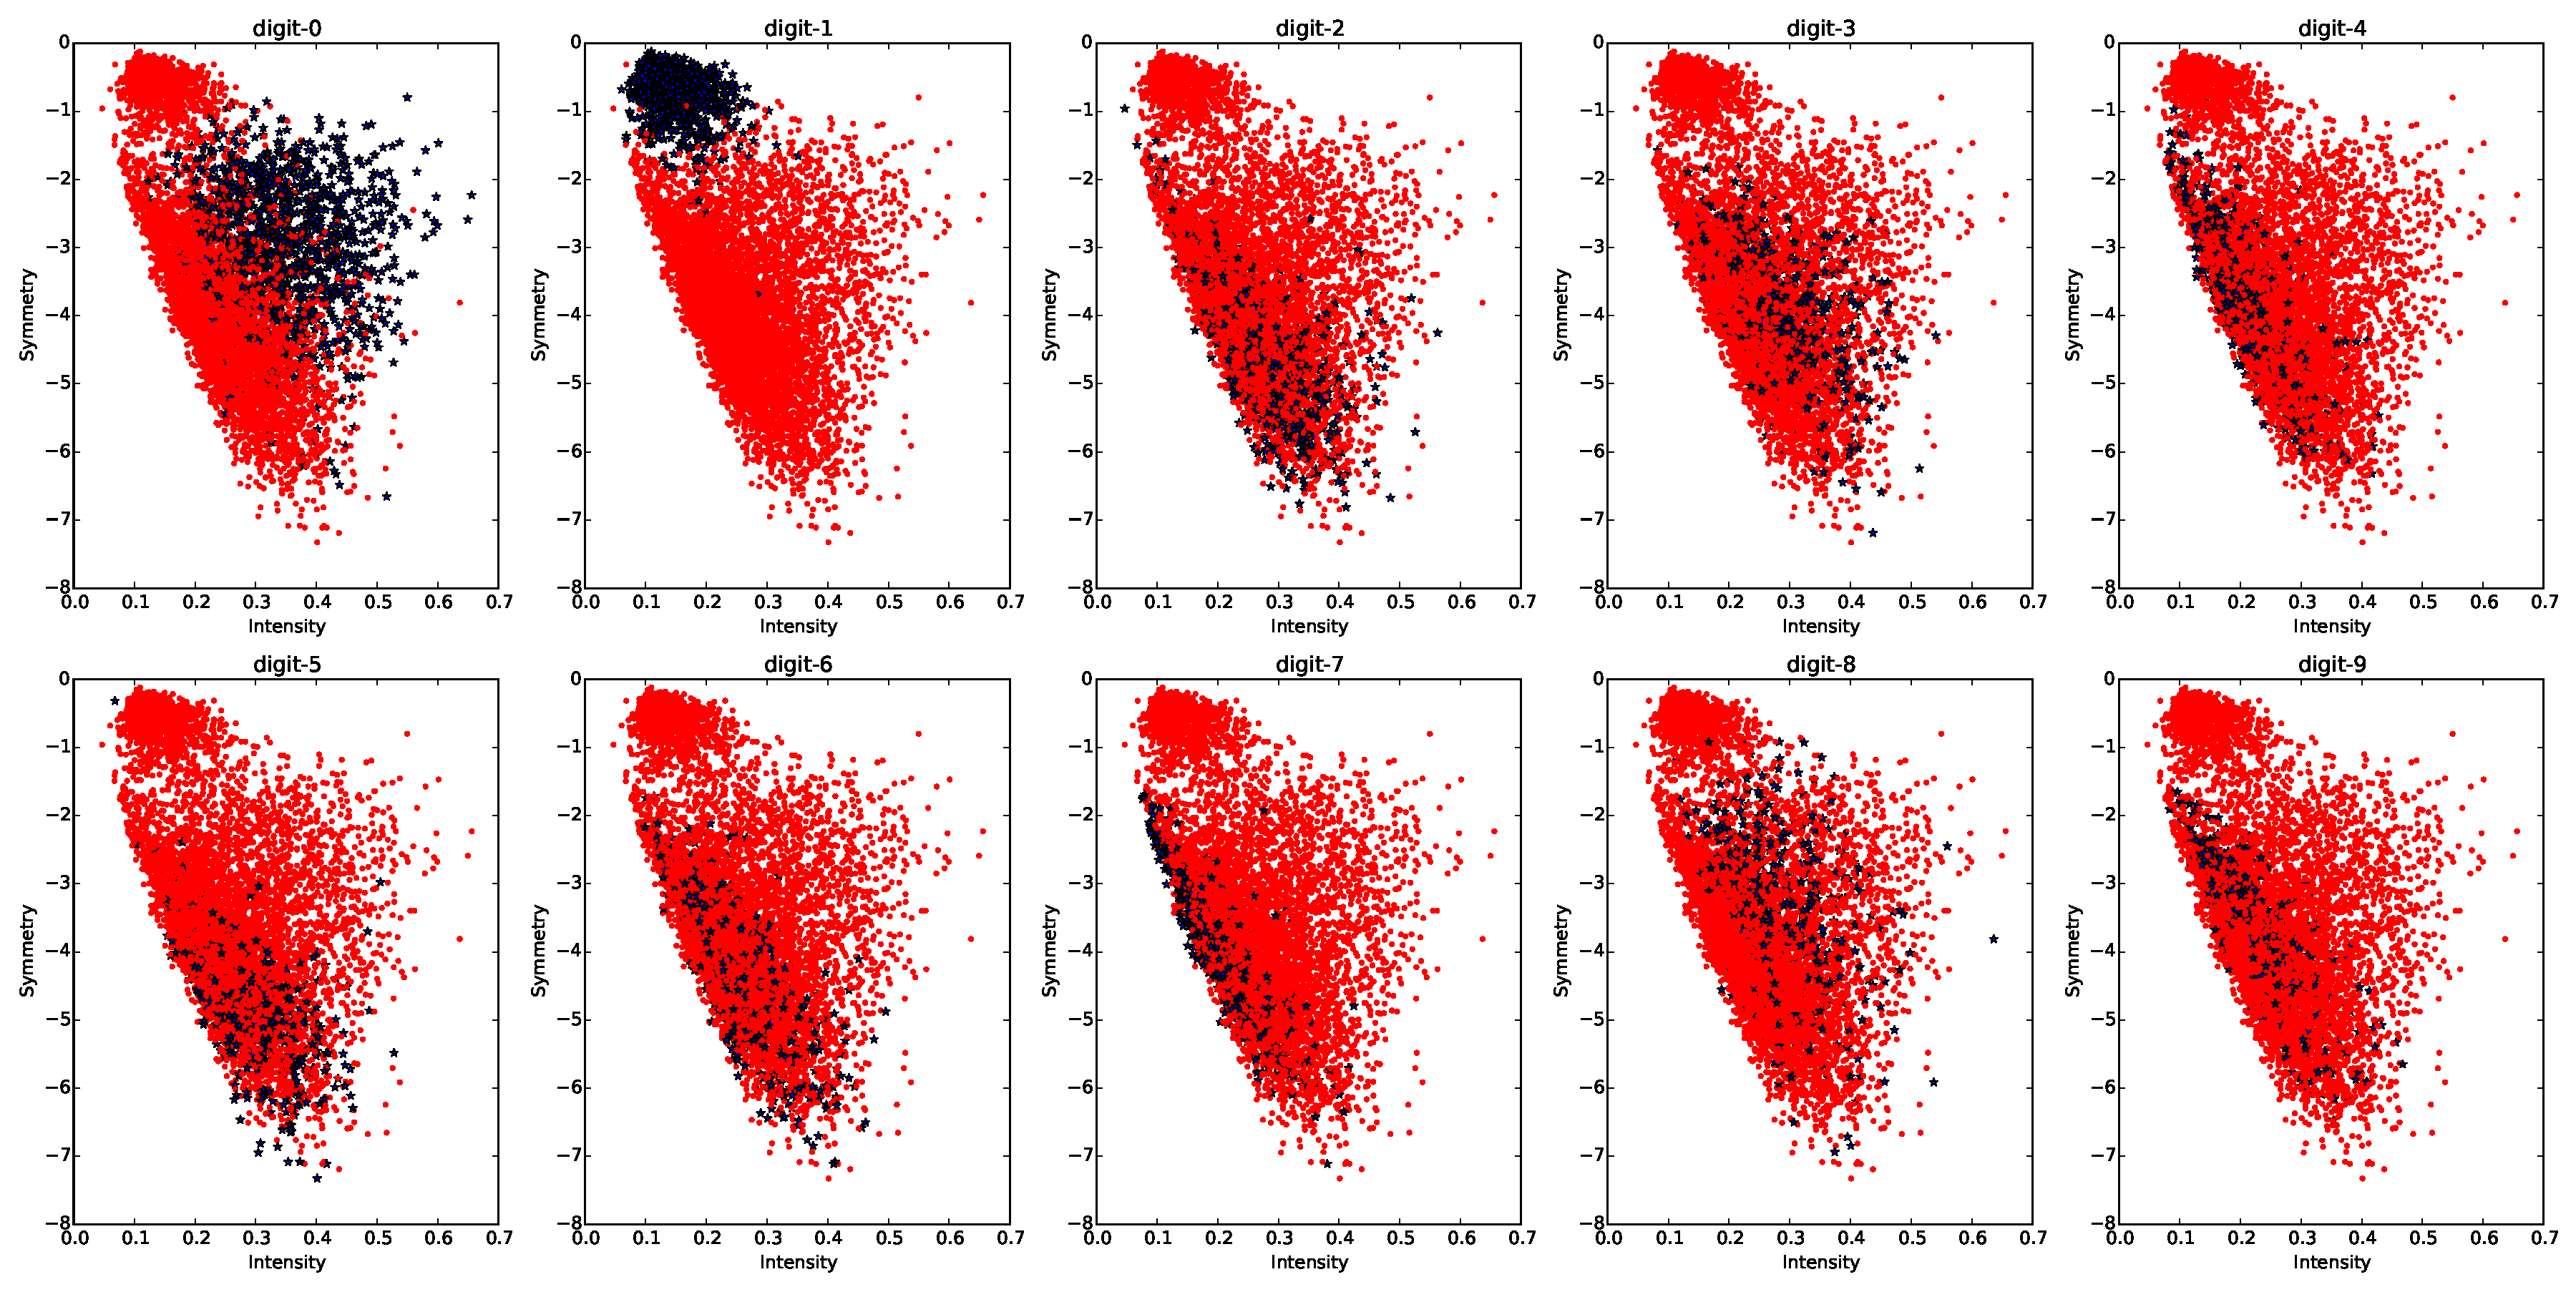
\includegraphics[width=6.3in]{digits.pdf}
\caption{Distributions of Digits}
\label{fig:digits}
\end{figure}

To build the linear regression model, the following optimization problem is solved,
\begin{equation*}
\min_\mathbf{x}\frac{1}{2}\|\mathbf{Ax-b}\|^2,
\end{equation*}
where $\mathbf{A}$ and $\mathbf{b}$ are defined based on the digit to classify from the rest. The tasks defined are to separate digits from the rest, namely, classifying digit $d$ and the rest, $d={0,\ldots,9}$. For $d=3$, for instance, $\mathbf{A}=[\tilde{\mathbf{A}},\mathbf{1}]\in\mathbb{R}^{7291\times3}$, where the number of 7291 is the total data samples in the data, and the first two columns represent \emph{intensity} and \emph{symmetry} of a sample, respectively; the elements in $\mathbf{b}$ are equal to 1 if in the training data, the data points have a label of 3, and equal to -1 otherwise.

\algorithm The following algorithms are implemented to solve the unconstrained optimization problem:
\begin{itemize}
  \item Steepest descent using constant stepsize rule where $\alpha$'s are randomly selected between 0 and 1
  \item Steepest descent using diminishing stepsize rule where $\alpha_r$'s revolve by the iteration, $r$, as $\frac{1}{r}$, $\frac{1}{r^2}$ and $\frac{1}{\sqrt{r}}$, respectively
  \item Steepest descent using Armijo rule where parameters are uniformly chosen with the policy $0.1<s<1.1$, $0.1<\beta<1$ and $0.1<\sigma<0.5$
\end{itemize}

All the implemented algorithms choose the same initial solution $\mathbf{x}^0$ as a starting point; the $\mathbf{x}^{r+1}$ is updated according the steepest decent methods with desired stepsize rules until either the maximum number of iterations has been reached or the objective values cannot be updated.

\result The first task performed is to separate digit "4" from the rest, and the performance of different algorithms is shown in Fig. \ref{fig:digit4}. Except the Armijo-rule-based algorithms, others diverge in less than 75 iterations. The optimal solution to the problem can be obtained by $\mathbf{x}=(\mathbf{A}\mathbf{A}^T)^{-1}\mathbf{A}\mathbf{b}$; Both algorithms that converge achieve values a little higher than the objective value of 1133.110. Tasks to classify other digits from the rest were also performed, giving similar results (i.e., only the last two algorithms converge). The resulting figures are included in the submitted zipped folder.
\begin{figure}[!tb]
\centering
\includegraphics[width=6.3in]{digit-4_rest.pdf}
\caption{Objective Reduction when Classifying Digit "4" and the Rest}
\label{fig:digit4}
\end{figure}

%One other task was carried out to classify digit "7" from "6". The , $\frac{0.1}{r}$, $\frac{0.1}{r^2}$ and $\frac{0.1}{\sqrt{r}}$
\analysis Table \ref{stepsize2} presents the evolution of stepsize in differen algorithms for classifying digit "4" and the rest. The Armijo-based methods effectively choose moderate stpesizes at each steps so that the objective values sufficiently descend. On the other hand, a step size greater than 0.0003 could be too big to lead the algorithms to converge.

Overall, the Armijo stepsize rules usually can efficiently reach the optimal solution or solutions that close to optimality. I also tried other experiments with different constant stepsizes; sometimes it converges but not very often. The stepsize needs to be selected carefully.
% Please add the following required packages to your document preamble:
% \usepackage{graphicx}
\begin{table}[!tb]
\centering
\caption{Stepsize Evolution in Problem 2}
\label{stepsize2}
\renewcommand{\arraystretch}{1.2}
\resizebox{\textwidth}{!}{%
\begin{tabular}{|c|c|c|c|c|c|c|c|}
\hline
                       & \textbf{Constant-0.01} & \textbf{Constant-0.429} & \textbf{Diminishing-1} & \textbf{Diminishing-2} & \textbf{Diminishing-1/2} & \textbf{Armijo-0.875/0.706/0.454} & \textbf{Armijo-1.039/0.711/0.114} \\ \hline
\textbf{Iteration 1}   & 1.000e-2               & 4.289e-1                & 1                      & 1                      & 1                        & 8.763e-6                          & 1.363e-5                          \\ \hline
\textbf{Iteration 2}   & 1.000e-2               & 4.289e-1                & 5.000e-1               & 2.500e-1               & 7.071e-1                 & 8.763e-6                          & 1.363e-5                          \\ \hline
\textbf{Iteration 3}   & 1.000e-2               & 4.289e-1                & 3.333e-1               & 1.111e-1               & 5.774e-1                 & 2.869e-4                          & 1.363e-5                          \\ \hline
\textbf{...}           & ...                    & ...                     & ...                    & ...                    & ...                      & ...                               & ...                               \\ \hline
\textbf{Iteration I-2} & 1.000e-2               & 4.289e-1                & 2.500e-2               & 1.984e-4               & 1.690e-1                 & 8.763e-6                          & 1.363e-5                          \\ \hline
\textbf{Iteration I-1} & 1.000e-2               & 4.289e-1                & 2.439e-2               & 1.929e-4               & 1.667e-1                 & 2.024e-4                          & 2.694e-5                          \\ \hline
\textbf{Iteration I}   & 1.000e-2               & 4.289e-1                & 2.381e-2               & 1.877e-4               & 1.644e-1                 & 8.763e-6                          & 1.916e-5                          \\ \hline
\end{tabular}
}
\end{table}
%\appendix
%\section{some contents}
%eee
\end{document}
